\documentclass{beamer}
\usetheme{Darmstadt}
\useinnertheme{rectangles}
\definecolor{garnet}{RGB}{114,47,55}
\definecolor{darkgarnet}{RGB}{80,30,37}
\definecolor{darkdarkgarnet}{RGB}{57,23,27}
\definecolor{darkdarkdarkgarnet}{RGB}{40,15,18}
\definecolor{gold}{RGB}{212,175,55}
\definecolor{darkgold}{RGB}{150,115,45}
\setbeamercolor{palette primary}{bg=garnet}
\setbeamercolor{palette secondary}{bg=darkgarnet} 
\setbeamercolor{palette tertiary}{bg=darkdarkgarnet}
\setbeamercolor{palette quaternary}{bg=darkdarkdarkgarnet}
\setbeamercolor{background canvas}{bg=white}
\setbeamercolor*{item}{fg=darkgold}
\setbeamercolor{block title}{bg=darkgold}


\title[TAB v2] % (optional, only for long titles)
{The Tagless Access Buffer (TAB)}
\subtitle{An Updated Approach to Reduce Cache Energy Usage with Minimal ISA Changes}
\author{Carlos Sanchez}
\institute[FSU]
{Computer Science Department\\ Florida State University}
\date{Fall 2015}
\subject{Computer Science}

\begin{document} 
\frame{\titlepage} 
\section{Initial pokings}
\subsection{How to do things?}
\begin{frame}{This is the first slide}
   Some content and whatever.
   How do you do bullets?
   How do you do images?
\end{frame}
\subsection{Some revelations}
\begin{frame}{This is the second slide}
   \framesubtitle{Doing some other cool stuff}
   You can only have one subtitle (so IDK when to use it)
   boring content
   extra boring content
\end{frame}
\section{First tests}
\subsection{Lists}
\begin{frame}{Some lists}
   \begin{itemize}
      \item This is a bullet list (begin\{itemize\})
      \item It works just like any other bullet list in latex
      \item That's nice
   \end{itemize}
   \begin{enumerate}
      \item This is a numbered list (begin\{enumerate\})
         \begin{enumerate}
            \item A subitem
            \item Another subitem
         \end{enumerate}
      \item This also works like other latex enumerations
   \end{enumerate}
   \begin{description}
      \item[First] The first item in a begin\{description\}
      \item[Second] The second item
      \item[Third] The third etc \ldots
   \end{description}
\end{frame}
\subsection{Images}
\begin{frame}{How it works}
   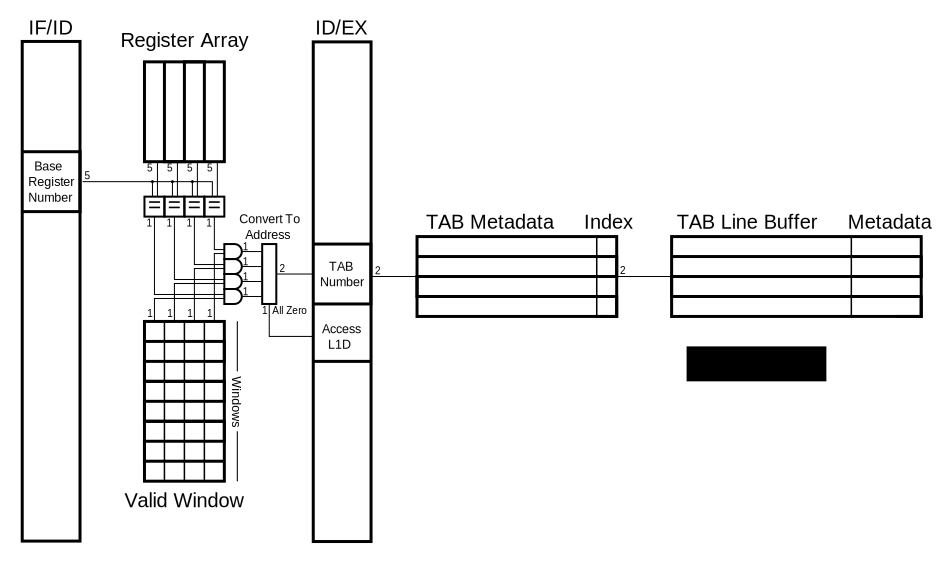
\includegraphics[width=\textwidth]{figures/tabhardware.pdf}
\end{frame}
\begin{frame}{How it works with explanation}
   \begin{columns} %[c] for centered, [T] for top
      \column{.5\textwidth}
      This is how it works: yeah
      \begin{block}{This is a block}
      A detailed explanation with a fancy header
      \end{block}
      \column{.5\textwidth}
      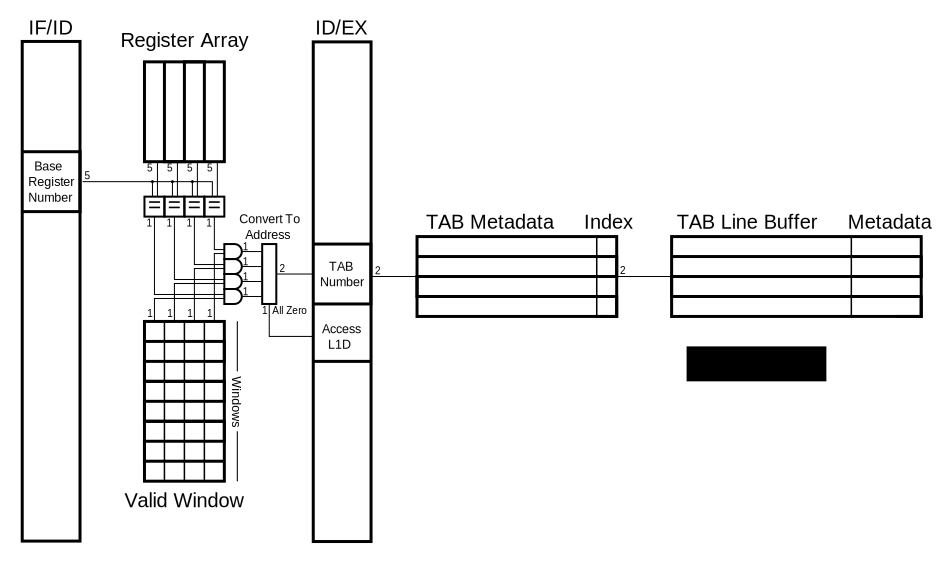
\includegraphics[width=\textwidth]{figures/tabhardware.pdf}
   \end{columns}
\end{frame}
\begin{frame}{How it works with explanation 2}
   \begin{columns} %[c] for centered, [T] for top
      \column{.5\textwidth}
         This is how it works: yeah
      \begin{block}{This is a block}
         A detailed explanation with a fancy header
      \end{block}
      \column{.5\textwidth}
      \begin{block}{An image in a block}
         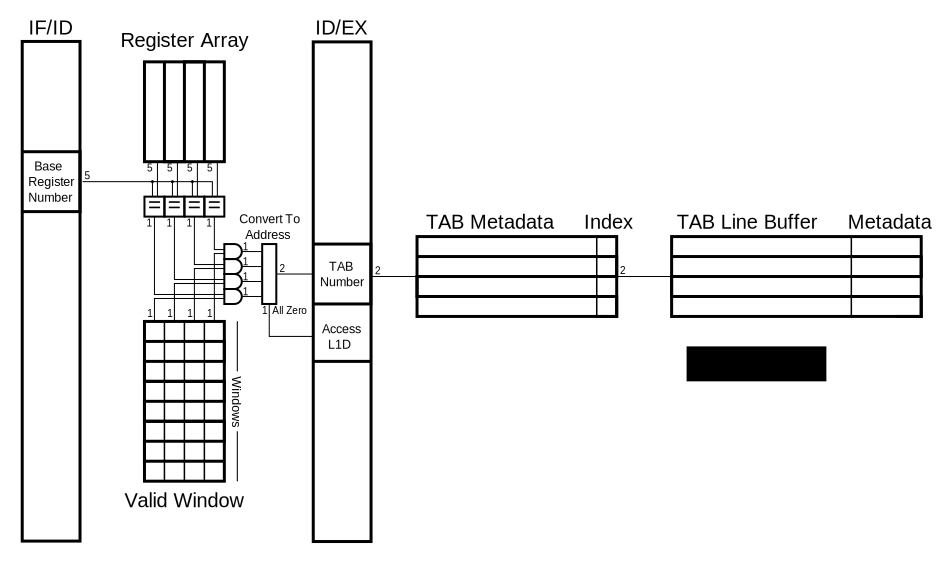
\includegraphics[width=\textwidth]{figures/tabhardware.pdf}
      \end{block}
   \end{columns}
\end{frame}
\end{document}
